%--------------------------------------------------------%
%______//------             GAC            ------\\______%
%______||------         Chapitre 5         ------||______%
%______\\------ Intro à la topo algébrique ------//______%
%--------------------------------------------------------%

\chapter{Introduction à la topologie algébrique}

  À tout espace topologique $X$ raisonnable, on associe des groupes.

  Une propriété fondamentale est qu'à toute application continue $f: X \to Y$ correspond un homomorphisme de
  groupes $f_\ast:F(X) \to F(Y)$.

  \section{Groupe fondamental d'un espace topologique}
  \label{sec:grp-fondamental-esp-topo}

    \subsection{Lacets}

    \begin{defi}
      Soit $X$ un espace topologique. Un \emph{arc} dans $X$ est une application continue $\gamma: [0,1] \to
      X,\, t \mapsto \gamma(t)$, où $\gamma(0)$ est l'\emph{origine} de $\gamma$ et $\gamma(1)$ est
      l'\emph{extrémité} de $\gamma$.
    \end{defi}

    
    Un arc peut être inversé:
      \[\check{\gamma}(t) = \gamma(1-t).\]
    Deux arcs $\gamma, \delta$ peuvent être composés si l'origine de $\delta$ est l'extrémité de $\gamma$. 
      \[(\gamma\delta)(t) =
      \begin{cases}
        \gamma(2t) & \text{si } 0 \leq t \leq \frac{1}{2},\\
        \delta(2t-1) & \text{si } \frac{1}{2} \leq t \leq 1.
      \end{cases}
      \]
    Pour avoir une composition toujours bien définie, on se restreint aux \emph{lacets}, c'est-à-dire les arcs
    tels que $\gamma(0) = \gamma(1) = x_0$. Si $x_0 = \gamma(0) = \gamma(1)$, on dit que $\gamma$ est
    \emph{basée en $x_0$}.

    En 1901, \textsc{Poincaré} (1854-1912) a eu l'idée que, si on regarde les lacets à déformation continue
    près, on obtient un groupe, qui détecte la présence de ``trous'' dans $X$.

    \begin{defi}
      Soient $\gamma_0$, $\gamma_1$ deux lacets basés en $x_0$. Une \emph{homotopie} de $\gamma_0$ à
      $\gamma_1$ est une application continue
        \[
          F:  [0,1] \times [0,1] \to X\\
        \]
      telle que
        \[
        \begin{cases}
          F(0,t) = \gamma_0(t), & \forall t \in [0,1],\\
          F(s,0) = F(s,1) = x_0, & \forall s \in [0,1], \\
          F(1,t) = \gamma_1(t), & \forall t \in [0,1].
        \end{cases}
        \]
    \end{defi}

    \begin{figure}[h]
      \centering
      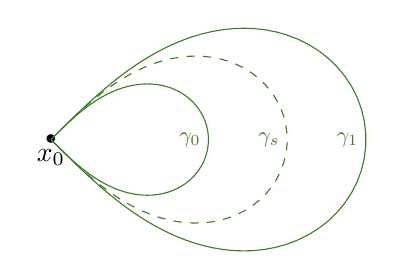
\begin{tikzpicture}
        \draw (0,0) node[scale=0.8]{$\bullet$} node[below]{$x_0$};
        \draw[color = OliveGreen] plot[domain={-pi/2}:{pi/2}, samples = 80] ({((2*cos(\x r))/(1+sin(\x r)*sin(\x r)))},%
                                                        {((2*sin(\x r)*cos(\x r)/(1+sin(\x r)*sin(\x r))))});
        \draw[color = OliveGreen, dashed] plot[domain={-pi/2}:{pi/2}, samples = 80] ({((3*cos(\x r))/(1+sin(\x r)*sin(\x r)))},%
                                                        {((3*sin(\x r)*cos(\x r)/(1+sin(\x r)*sin(\x r))))});
        \draw[color = OliveGreen] plot[domain={-pi/2}:{pi/2}, samples = 80] ({((4*cos(\x r))/(1+sin(\x r)*sin(\x r)))},%
                                                        {((4*sin(\x r)*cos(\x r)/(1+sin(\x r)*sin(\x r))))});
        \draw (2, 0) node[color = OliveGreen, left, scale = 0.8]{$\gamma_0$};
        \draw (3, 0) node[color = OliveGreen, left, scale = 0.8]{$\gamma_s$};
        \draw (4, 0) node[color = OliveGreen, left, scale = 0.8]{$\gamma_1$};
      \end{tikzpicture}
      \caption{Exemple d'homotopie}
      \label{fig:exemple-homotopie}
    \end{figure}

    Si on pose $\gamma_s(t) = F(s,t)$, on voit que $(\gamma_s)_{s \in [0,1]}$ est une famille continue de
    lacets qui interpole entre $\gamma_0$ et $\gamma_1$.

    \begin{defi}
      Deux lacets $\gamma_0$ et $\gamma_1$ (basés en $x_0$) sont \emph{homotopes} s'il existe une homotopie de
      $\gamma_0$ à $\gamma_1$, et dans ce cas on écrit $\gamma_0 \sim \gamma_1$. On écrit le lacet trivial
      basé en $x_0$ $\epsilon_{x_0}$. Si $\gamma \sim \epsilon_{x_0}$, on dit que $\gamma$ est homotope à zéro.
    \end{defi}

    \begin{prop}
      Pour les lacets basés en $x_0 \in X$, la relation ``être homotope'' est une relation d'équivalence. On
      note $[\gamma]$ la classe d'équivalence de $\gamma$.
    \end{prop}

    \begin{preuve}
      Exercice.
    \end{preuve}

    \begin{figure}[h]
      \centering
      \begin{tikzpicture}
        \draw (0,0) node[scale=0.8]{$\bullet$} node[below]{$x_0$};
        \begin{scope}[rotate=30]
        \draw[color = OliveGreen] plot[domain={pi/2}:{3*pi/2}, samples = 80] ({((4*cos(\x r))/(1+sin(\x r)*sin(\x r)))},%
                                                        {((4*sin(\x r)*cos(\x r)/(1+sin(\x r)*sin(\x r))))});
        \end{scope}
        \begin{scope}[rotate=40]
        \draw[color = OliveGreen] plot[domain={-pi/2}:{pi/2}, samples = 80] ({((2*cos(\x r))/(1+sin(\x r)*sin(\x r)))},%
                                                        {((2*sin(\x r)*cos(\x r)/(1+sin(\x r)*sin(\x r))))});
        \end{scope}
        \draw (-5, 3) rectangle (3, -4);
        \draw (-5, 3) node[below right] {$X$};
        \draw (-2, -1.5) circle(0.5);
      \end{tikzpicture}
      \caption{Exemple d'homotopies ayant des classes d'équivalence différentes (le rond est un ``trou'')}
      \label{fig:exemple-homotopie-classes-equiv}
    \end{figure}

    
    \subsection{Groupe fondamental}

    \begin{theo}[-définition] \index{Groupe!Fondamental}
      On note $\Pi_1(X, x_o)$ l'ensemble des classes d'homotopie des lacets de $X$ basés en $x_o$. Avec la
      multiplication $[\gamma][\delta] = [\gamma \delta]$, $\Pi_1(X, x_0)$ est un groupe, appelé \emph{groupe
        fondamental} de $X$ (en $x_0$).

      L'élément neutre est $[\epsilon_{x_0}]$ et l'inverse de $[\gamma]$ est $[\check{\gamma}]$.
    \end{theo}

    \begin{preuve}
      On vérifie d'abord que, si $\gamma_0 \sim \gamma_1$, $\delta_0 \sim \delta_1$ alors $\gamma_0\delta_0
      \sim \gamma_1\delta_1$, c'est-à-dire que la multiplication est bien définie. On a donc que $[\gamma_0] =
      [\gamma_1]$ et $[\delta_0 = \delta_1] \Rightarrow [\gamma_0 \delta_0] = [\gamma_1 \delta_1]$. 

      Soient $F$ et $G$ deux homotopies de $\gamma_0$ à $\gamma_1$ et de $\delta_0$ à $\delta_1$
      respectivement. Une homotopie de $\gamma_0\delta_0$ à $\gamma_1\delta_1$ est donnée par 
        \[
        H(s,t) = 
        \begin{cases}
          F(s,2t) & \text{si } 0 \leq t \leq \frac{1}{2},\ s \in [0,1]\\
          G(s, 2t-1) & \text{si } \frac{1}{2} \leq t \leq 1,\ s \in [0,1]
        \end{cases}
        \]
      (à vérifier).

      Il faut encore montrer que:
      \begin{itemize}
      \item $\epsilon_{x_o}\gamma \sim \gamma \sim \gamma \epsilon_{x_0}$;
      \item $\gamma \check{\gamma} \sim \epsilon_{x_0}$;
      \item associativité: si $\gamma_0$, $\gamma_1$, $\gamma_2$ sont trois lacets basés en $x_0$,
        $\gamma_0(\gamma_1\gamma_2) \sim (\gamma_0\gamma_1)\gamma_2$.
      \end{itemize}
    \end{preuve}



    \subsection{Propriétés du groupe fondamental}

    \paragraph{Rappel:} Un espace est \emph{connexe par arcs} si deux points peuvent être joints par un arc.

    \begin{prop}\index{Connexe!par arcs}
      Si $X$ est connexe par arc, alors 
        \[\Pi_1(X, x_0) \cong \Pi_1(X, y_0)\ \forall x_0, y_0 \in X.\]
    \end{prop}
    
    \begin{conseq}
      Si $X$ est connexe par arcs, on peut parler du \emph{groupe fondamental de $X$}, noté $\Pi_1(X)$.
    \end{conseq}


    \begin{preuve}
      Exercice. Dessin de l'idée de la preuve:
      \begin{center}
        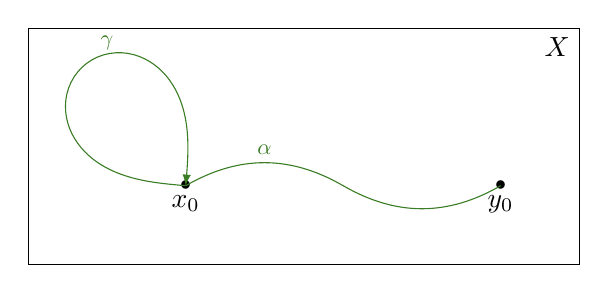
\begin{tikzpicture}
          \draw (-2, 2) rectangle (5, -1);
          \draw (5, 2) node[below left]{$X$};
          \draw (0,0) node[scale=0.8]{$\bullet$} node[below]{$x_0$};
          \draw (4,0) node[scale=0.8]{$\bullet$} node[below]{$y_0$};
          \begin{scope}[rotate=-50]
            \draw[color = OliveGreen, ->, >=latex] plot[domain={pi/2}:{3*pi/2}, samples = 80] ({((2*cos(\x
              r))/(1+sin(\x r)*sin(\x r)))}, {((2*sin(\x r)*cos(\x r)/(1+sin(\x r)*sin(\x r))))});
          \end{scope}
            \draw[color = OliveGreen](-1, 2) node[below, scale=0.8]{$\gamma$};
          \draw[color = OliveGreen] (0,0) to[bend left] node[midway, above, scale = 0.8]{$\alpha$} (2, 0)
          to[bend right] (4,0);
        \end{tikzpicture}
      \end{center}
      Ainsi pour passer de $\gamma \in \Pi_1(X, x_0)$ à un élément de $\Pi_1(X, y_0)$, on prend
      $\check{\alpha}\gamma \alpha$.
    \end{preuve}
    
    \begin{defi} \index{Connexe!simplement}
      Un espace $X$ (connexe par arcs) est \emph{simplement connexe} si $\Pi_1(X) = 0$ (ou
      $\{1\}$). C'est-à-dire que tout lacet dans $X$ est homotope à $\epsilon_{x_0}$.
    \end{defi}
    

    \begin{exs}
      \begin{enumerate}
      \item Un tel ensemble de $\R^n$ est simplement connexe:
        \begin{center}
        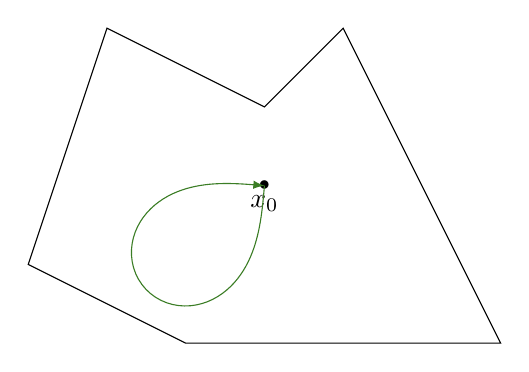
\begin{tikzpicture}
          \draw (0,0) node[scale=0.8]{$\bullet$} node[below]{$x_0$};
          \begin{scope}[rotate=40]
            \draw[color = OliveGreen, ->, >=latex] plot[domain={pi/2}:{3*pi/2}, samples = 80] ({((2*cos(\x
              r))/(1+sin(\x r)*sin(\x r)))}, {((2*sin(\x r)*cos(\x r)/(1+sin(\x r)*sin(\x r))))});
          \end{scope}
            \draw (2,0) -- (3, -2) -- (-1, -2) -- (-3, -1) -- (-2, 2) -- (0, 1) -- (1, 2) -- cycle;
        \end{tikzpicture}
      \end{center}
      \item Les arbres sont simplements connexes:
        \begin{center}
          \begin{tikzpicture}
            \draw (-1, -1) -- (0,0) -- (1, -1) -- (0,0) -- (1.5, 2) -- (2.5, 1) -- (1.5, 2) -- (2, 3) -- (1,
            4) -- (2, 3) -- (3, 4);
            \draw[color = OliveGreen!80] (0,0) node[scale = 0.8]{$\bullet$};
            \draw[color = OliveGreen!80] (-1,-1) node[scale = 0.8]{$\bullet$};
            \draw[color = OliveGreen!80] (1,-1) node[scale = 0.8]{$\bullet$};
            \draw[color = OliveGreen!80] (1.5,2) node[scale = 0.8]{$\bullet$};
            \draw[color = OliveGreen!80] (2.5,1) node[scale = 0.8]{$\bullet$};
            \draw[color = OliveGreen!80] (2,3) node[scale = 0.8]{$\bullet$};
            \draw[color = OliveGreen!80] (1,4) node[scale = 0.8]{$\bullet$};
            \draw[color = OliveGreen!80] (3,4) node[scale = 0.8]{$\bullet$};
          \end{tikzpicture}
        \end{center}
      \item L'ensemble suivant est homéomorphe à $[0,1] \times [0,1]$.
        \begin{center}
          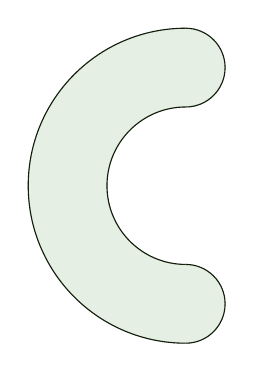
\begin{tikzpicture}
            \draw (0,0) arc(90:270:2);
            \draw (0,-1) arc(90:270:1);
            \draw (0, 0) arc(90:-90:0.5); 
            \draw (0, -3) arc(90:-90:0.5);
            \filldraw[color = OliveGreen!80, opacity = 0.15] (0,0) arc(90:270:2) arc(-90:90:0.5) 
            arc(270:90:1) arc(-90:90:0.5);
          \end{tikzpicture}
        \end{center}
      \item Pour $n \geq 2$, la sphère $\mathbb{S}^{n}$ est simplement connexe ($S^1$ n'est pas simplement connexe).
      \end{enumerate}
    \end{exs}

    \begin{prop}
      Soit $f: X \to Y$ une application continue, avec $y_0 = f(x_0)$. On pose $f_\ast: \Pi_1(X, x_0) \to
      \Pi_1(Y, y_0), [\gamma] \mapsto [f \circ \gamma]$. Alors $f_\ast$ est un homomorphisme de groupes.

      De plus, 
      \begin{enumerate}
      \item si $f:X \to Y$, $g: Y \to Z$ sont continues avec $y_0 = f(x_0)$ et $z_0 = g(y_0)$, alors $(g \circ
        f)_\ast = g_\ast \circ f_\ast$;
      \item $id_X : X \to X$, alors $(id_X)_\ast = Id_{\Pi_1(X, x_0)}$.
      \end{enumerate}
    \end{prop}

    \begin{preuve}
      Exercice.
    \end{preuve}

    \begin{theo}
      On a que
        \[\Pi_1(S^1) \cong \Z\]
    \end{theo}

    \begin{preuve}
      Difficile, et long.
    \end{preuve}

    \begin{exs}
      \begin{enumerate}
      \item Soit $\Pi^2$ le tore. En découpant le long de $a_1$ et $a_2$, on obtient un carré. Ceci montre que
        $[a_1a_2a_1^{-1}a_2^{-1}] = 1$ dans $\Pi_1(\Pi^2)$. Ainsi $\Pi_1(\Pi^2) = \Z^2$.

        Si on enlève à $\Pi^2$ un petit disque ouvert $D$, le bord de $D$ est $a_1a_2a_1^{-1}a_2^{-1}$ dans
        $\Pi_1(X)$, où $X = \Pi^2 \setminus D$. En fait, $\Pi_1(X) \cong \F_2 = \langle a_1, a_2 \rangle$
        ($\F_2$ est le groupe libre). 

        
        \begin{center}
          \begin{tikzpicture}
            \draw plot[domain = 0:2*pi, samples = 80]({5*cos(\x r)}, {3*sin(\x r)});
            \draw plot[domain = pi:2*pi, samples = 80]({3*cos(\x r)}, {1*sin(\x r)+0.6});
            \draw plot[domain = 0:pi, samples = 80]({2*cos(\x r)}, {0.5*sin(\x r)-0.15});
            % % TO ADD: cercles générateurs du tore + petit cercle à enlever
          \end{tikzpicture}
        \end{center}

      \item On a que $\Pi_1(\Sigma_2) = \langle a_1, a_2, b_1, b_2 | [a_1, a_2][b_1, b_2] = 1 \rangle$.
        \begin{center}
          \begin{tikzpicture}
            % TODO: Dessiner double tore
          \end{tikzpicture}
        \end{center}
      \end{enumerate}
    \end{exs}

  \section{Produits libres}
  \label{sec:produits-libres}

  \begin{defi} \index{Produit libre}
    Soient $A$ et $B$ deux groupes. Le \emph{produit libre}, noté $G = A \ast B$ est l'ensemble des mots de la
    forme
      \[a_1b_1a_2b_2 \cdots a_kb_k,\ k \in \N,\ a_i \in A,\ b_i \in B\]
    et $a_2, \ldots, a_k \neq \epsilon_A$ et $b_1, \ldots, b_{k-1} \neq \epsilon_B$. 
  \end{defi}

  Donc $G$ est l'ensemble des mots obtenus en alternant un élément non trivial d'un groupe, un élément non
  trivial de l'autre, etc.

  \begin{ex}
    \begin{enumerate}
    \item $\Z \ast \Z = \F_2 = \langle a, b \rangle$.

    \item En général, $\F_k \ast \F_m \cong \F_{k+m}$.

    \item Soit $D_\infty$ le groupe dihédral infini, c'est le sous-groupe des isométries de $\R$ engendré par
      deux symétries centrales. Alors
        \[D_\infty \cong \Z/2\Z \ast \Z/2\Z\]
      où $\Z/2\Z = \langle s_1 \rangle$ et $\Z/2\Z = \langle s_2 \rangle$. En effet, prenons
      \begin{center}
        \begin{tikzpicture}
          \draw[->, >=latex] (-5, 0) -- (5,0) node[right]{$\R$};
          \draw (-2, 0) node[scale=0.8]{$\bullet$} node[above left]{$-1$};
          \draw (2, 0) node[scale=0.8]{$\bullet$} node[above right]{$1$};
          \draw (0,0.2) -- (0, -0.2);
          \draw (0,0) node[above right]{$0$};
          \draw[dashed, color = OliveGreen!80] (-2, 1) -- (-2, -1);
          \draw[dashed, color = OliveGreen!80] (2, 1) -- (2, -1);
          \draw[<->, >=latex, color = OliveGreen!80] (-3, 0) to[bend right] node[midway, below left]{$s_1$} (-1, 0);
          \draw[<->, >=latex, color = OliveGreen!80] (1, 0) to[bend right] node[midway, below right]{$s_2$} (3, 0);
        \end{tikzpicture}
      \end{center}
      On voit que pour tout $s_{i_1} \cdots s_{i_k}$ avec $i_j \neq i_{j+1}$, on a $s_{i_1} \cdots s_{i_k}
      \neq 0$, ainsi $s_{i_1} \cdots s_{i_k} \neq \epsilon_{D_\infty}$.
    \end{enumerate}
  \end{ex}

  \begin{lem}[du Ping-Pong, 2ème version] \index{Lemme!du Ping-Pong!2nde version}
    Soient $G_1, G_2$ des sous-groupes de $Sym(X)$. On suppose que $|G_1| \geq 2$, $|G_2| \geq 3$. S'il existe
    deux parties $A_1, A_2 \subset X$ telles que $A_i \neq \varnothing$, $A_1 \not\subset A_2$ avec 
    \begin{itemize}
    \item $g_1(A_1) \subseteq A_2 \forall g_1 \in G_1 \setminus \{id\}$;
    \item $g_2(A_2) \subseteq A_1 \forall g_2 \in G_2 \setminus \{id\}$,
    \end{itemize}
    alors le sous-groupe engendré par $G_1 \cup G_2$ dans $Sym(X)$ est isomorphe à $G_1 \ast G_2$.
  \end{lem}

  \section{Théorème de Van Kampen (version simple)}

  \begin{theo}[de Van Kampen] \index{Théorème!de Van Kampen}
    Soit $X$ un espace connexe par arcs. On suppose que $X = U \cup V$ où 
    \begin{itemize}
    \item $U$ et $V$ sont des ouverts connexes par arcs;
    \item $U \cap V$ est simplement connexe et non vide.
    \end{itemize}
    Alors $\Pi_1(X) \cong \Pi_1(U) \ast \Pi_1(V)$ (produit libre des groupes fondamentaux).
  \end{theo}

  \begin{exs} \index{Bouquet!à deux cercles} \index{Bouquet!à $n$ cercles}
    \begin{enumerate}
    \item Le bouquet à deux cercles. Si $X = U \cup V$, on a $U \cap V = \{x\}$.
      \begin{center}
        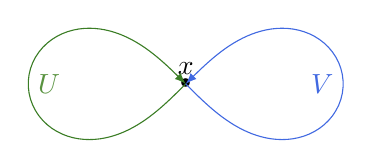
\begin{tikzpicture}
          \draw (0,0) node[scale=0.8]{$\bullet$} node[above]{$x$};
          \draw[color = OliveGreen, ->, >=latex] 
               plot[domain={pi/2}:{3*pi/2}, samples = 80] 
                   ({((2*cos(\x r))/(1+sin(\x r)*sin(\x r)))}, {((2*sin(\x r)*cos(\x r)/(1+sin(\x r)*sin(\x r))))});
           \draw[color = RoyalBlue, ->, >=latex] 
               plot[domain={-pi/2}:{pi/2}, samples = 80] 
                   ({((2*cos(\x r))/(1+sin(\x r)*sin(\x r)))}, {((2*sin(\x r)*cos(\x r)/(1+sin(\x r)*sin(\x r))))});
           \draw[color = OliveGreen!80] (-2, 0) node[right]{$U$};
           \draw[color = RoyalBlue] (2, 0) node[left]{$V$};
        \end{tikzpicture}
      \end{center}
      Le groupe fondamental est
        \[\Pi_1(X) = \Pi_1(U) \ast \Pi_1(V) = \Z \ast \Z = \F_2.\]

      \item Si $(X, x_o)$ et $(Y, Y_0)$ sont deux espaces pointés (car on a donné des points), le
        \emph{wedge} ou \emph{joint} de $X$ et $Y$ est $X \wedge Y = X \cupdot Y / x_0=y_0$. Si $x_0, y_0$
        possèdent des voisinages simplement connexes, alors
          \[\Pi_1(X \wedge Y) = \Pi_1(X, x_0) \ast \Pi_1(Y, y_0).\]
        Par exemple si on prend $X = S^1$ et $Y = \Pi^2$, on obtient la chose suivante pour $X \wedge Y$.

        \begin{center}
          \begin{tikzpicture}
            \draw plot[domain = 0:2*pi, samples = 80]({5*cos(\x r)}, {3*sin(\x r)});
            \draw plot[domain = pi:2*pi, samples = 80]({3*cos(\x r)}, {1*sin(\x r)+0.6});
            \draw plot[domain = 0:pi, samples = 80]({2*cos(\x r)}, {0.5*sin(\x r)-0.15});
            \draw[color = OliveGreen] (-3, -1) node[scale = 0.8]{$\bullet$} node[below right]{$x_0 = y_0$};
            \draw[color=OliveGreen] (-3, 0) circle(1);
          \end{tikzpicture}
        \end{center}

      \item On appelle $B_n$ le bouquet de $n$ cercles. Alors
          \[\Pi_1(B_n) = \F_n = \langle a_1, \ldots, a_n\rangle. \]
        Plus généralement, si $X = (V,E)$ et un graphe connexe avec $n = |V|$, $m = |E|$ vu comme espace
        topologique en identifiant chaque arête à une copie de $[0,1]$, alors
          \[\Pi_1(X) \cong \F_{m-n+1}.\]
        Par exemple si $G$ est le graphe suivant:
        \begin{center}
          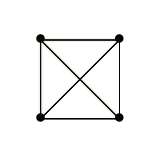
\begin{tikzpicture}
            \node[scale=0.8] (a) at (0,0) {$\bullet$};
            \node[scale=0.8] (b) at (1,0) {$\bullet$};
            \node[scale=0.8] (c) at (0,-1) {$\bullet$};
            \node[scale=0.8] (d) at (1,-1) {$\bullet$};
            \draw (a.center) -- (b.center) -- (c.center) -- (d.center) -- (a.center) -- (c.center);
            \draw (b.center) -- (d.center);
            \draw (a.center) -- (b.center) -- (c.center) -- (d.center) -- (a.center) -- (c.center);
            \draw (b.center) -- (d.center);
            \draw[color=OliveGreen, line width=1.5pt, opacity = 0.1] (c.center) -- (a.center) -- (b.center) --
            (a.center) -- (d.center);
          \end{tikzpicture}
        \end{center}
          \[\Pi_1(G) = \F_{6-4+1} = \F_3.\]
        En effet, soit $\mathcal{T}$ un \emph{arbre maximal} \index{Arbre!maximal} de $X$ (un \emph{arbre
          maximal} est un sous-graphe de $X$, sans circuit passant par tous les sommets). En contractant
        $\mathcal{T}$ sur un point, on obtient un bouquet à $m-n+1$ cercles, car $\mathcal{T}$ a $n-1$ arêtes.
        \begin{center}
          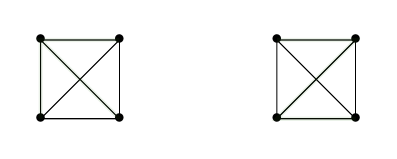
\begin{tikzpicture}
            \node[scale=0.8] (a) at (0,0) {$\bullet$};
            \node[scale=0.8] (b) at (1,0) {$\bullet$};
            \node[scale=0.8] (c) at (0,-1) {$\bullet$};
            \node[scale=0.8] (d) at (1,-1) {$\bullet$};
            \draw (a.center) -- (b.center) -- (c.center) -- (d.center) -- (a.center) -- (c.center);
            \draw (b.center) -- (d.center);
            \draw[color=OliveGreen, line width=1.5pt, opacity = 0.1] (c.center) -- (a.center) -- (b.center) --
            (a.center) -- (d.center);
            \begin{scope}[xshift = 3cm]
               \node[scale=0.8] (a) at (0,0) {$\bullet$};
               \node[scale=0.8] (b) at (1,0) {$\bullet$};
               \node[scale=0.8] (c) at (0,-1) {$\bullet$};
               \node[scale=0.8] (d) at (1,-1) {$\bullet$};
               \draw (a.center) -- (b.center) -- (c.center) -- (d.center) -- (a.center) -- (c.center);
               \draw (b.center) -- (d.center);
               \draw[color=OliveGreen, line width=1.5pt, opacity = 0.1] (a.center) -- (b.center) -- (c.center)
               -- (d.center);
            \end{scope}
          \end{tikzpicture}
        \end{center}
        Ci-dessus on a des arbres maximaux, car il reste 3 arêtes quand on contracte les arêtes vertes (on
        obtient donc un bouquet à 3 arêtes, dont le $\Pi_1$ est $\F_3$).
    \end{enumerate}
  \end{exs}




  \section{Revêtements}
  \label{sec:revetements}


  Tous les espaces sont supposés connexes par arcs et localement connexes par arcs.

  \begin{defi} \index{Revêtement}
    Un triplet $(X,Y,p)$, noté $\substack{Y\\\downarrow\\ X}p$ est un \emph{revêtement} de $X$ si: 
    \begin{itemize}
    \item $p$ est une application continue surjective $Y \to X$.
    \item Pour tout $x \in X$, $p^{-1}(X)$ est discret dans $Y$.
    \item Tout $x \in X$ possède un \emph{voisinage trivialisant} \index{Voisinage!trivialisant} $U_x$,
      c'est-à-dire un voisinage connexe par arcs tel que $p^{-1}(U_x)$ est homéomorphe à $p^{-1}(x) \times
      U_X$, par un homéomorphisme $h_x: p^{-1}(U_x) \to p^{-1} \times U_x$ tel que le diagramme suivant
      commute (où $p_2$ est la projection sur le 2ème facteur).
      \begin{center}
        \begin{tikzcd}[column sep = small]
          p^{-1}(U_x) \arrow[rr, "h_x"] \arrow[rd, "p \big|_{p^{-1}(U_x)}" below left] & & p^{-1}(x) \times U_x \\
          & U_x \arrow[ru, leftarrow, "p_2" below right] &
        \end{tikzcd}
      \end{center}
    \end{itemize}
    L'image mentale d'un revêtement est celle de la ``pile d'assiettes''.

    \begin{center}
      \begin{tikzpicture}
        \draw (-5, 0) -- (5, 0) node[right]{$X$};
        \draw (0,0) node[scale=0.8]{$\bullet$};
        \draw[color = OliveGreen, line width = 1.5pt, opacity = 0.1] (-1,0) to node[near end, below]{$U_x$} (1,0);
        \draw (-3.5, 3) arc(225:315:5) node[right]{$Y$};
        \foreach \x in {1,2,...,5} {
          \draw[color = RoyalBlue] (0,{1.5+(\x/2)}) node[scale=0.8]{$\bullet$};
          \draw[color = OliveGreen, line width = 1.5pt, opacity = 0.1] (-1,{1.5+(\x/2)}) -- (1,{1.5+(\x/2)});
        }
        \draw[color=RoyalBlue] (0, 2) node[below]{$p^{-1}(x)$};
        \draw[color=OliveGreen] (-1, 4) node[above]{$p^{-1}(U_x)$};
      \end{tikzpicture}
    \end{center}

    On dira que $\substack{Y\\\downarrow\\ X}p$ est un \emph{revêtement à $n$ feuillets} \index{Revêtement!à
      $n$ feuillets} si $\# p^{-1}(x) = n$, et a \emph{une infinité de feuillets} si $\# p^{-1}(x) = \infty$.
  \end{defi}

  
  \begin{exs}
    \begin{enumerate}
    \item Soit $X = \{z \in \C\ |\ |z| = 1 \}$. Alors l'espace $Y$ peut être représenté par une hélice, mais $Y
      = \R$. Alors $p: \R \to \S^1$ est défini par $p(t) = e^{2\pi i t}$ et $\substack{Y\\\downarrow\\ X}p$
      est un revêtement car $p$ est surjective. Si $z = e^{2\pi i \phi}$, alors $p^{-1}(z) = \phi + \Z$ est
      discret dans $\R$. Enfin, si $z = e^{2 \pi i \phi} \in S^1$, $U_z = S^1 \setminus \{-z\}$ (tout le
      cercle sauf le point opposé à $z$) est un voisinage de $z$, et $p^{-1}(U_z) = \R \setminus \{\phi +
      (2k+1)\pi, k \in \Z\} \cong \Z \times U_z$ car $\Z = p^{-1}(z)$. On ne prend pas les multiples impairs
      de $\pi$ car on ne veut pas $z+\pi, z-\pi, z+3\pi, \ldots$ dans le revêtement.

    \item Soit $X = S^1$, $Y = S^1$ et $p: S^1 \to S^1,\ z \mapsto z^n$ avec $n > 0$ et un revêtement à $n$
      feuillets. On parcourt le cercle $n$ fois, et on arête au même point qu'on a commencé.

    \item Si $x$ est un bouquet à deux boucles, alors $Y_{1,n}$ défini comme suit est un revêtement à $n$
      feuillets. $Y_{1, \infty}$ a une infinité de feuillets. $Y_2$ vu comme $\Z^2$ (le réseau à coordonnées
      entières) est aussi un revêtement à une infinité de feuillets.
    \end{enumerate}
  \end{exs}



  \begin{lem} \label{lem:lemme-A}
    Soit $\substack{Y\\\downarrow\\ X}p$ un revêtement. Soit $Z$ un espace connexe et soient $f_0, f_1 : Z
    \to Y$ deux applications continues avec $p \circ f_0 = p \circ f_1$. Alors $\{z \in Z | f_o(z) = f_1(z)\}
    = \varnothing$ ou $Z$.
    \begin{center}
      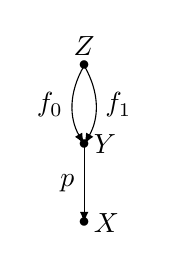
\begin{tikzpicture}
        \draw (0,0) node[scale=0.8]{$\bullet$} node[above]{$Z$};
        \draw (0,-1) node[scale=0.8]{$\bullet$} node[right]{$Y$};
        \draw (0, -2) node[scale=0.8]{$\bullet$} node[right]{$X$};
        \draw[->, >=latex] (0,0) to[bend right] node[midway, left] {$f_0$} (0, -1);
        \draw[->, >=latex] (0,0) to[bend left] node[midway, right] {$f_1$} (0, -1);
        \draw[->, >=latex] (0,-1) to node[midway, left] {$p$} (0, -2);        
      \end{tikzpicture}
    \end{center}
  \end{lem}

  \begin{preuve}
    Exercice.
    \begin{center}
      \begin{tikzpicture}[math3d]
        % Draw helix
        \draw [domain=-2*pi:2*pi, samples=80, smooth] plot ({cos(\x r)}, {sin(\x r)}, \x/pi) ;
        % Draw circle
        \draw (0,0, -4) circle(1);
        % Draw alpha on helix
        \draw [domain=0:pi, samples=80, smooth, color = OliveGreen!80, line width = 2pt] plot ({cos(\x r)},
        {sin(\x r)}, \x/pi) node[xshift = 0.5cm]{$\tilde{\alpha}$};
        % Draw alpha on circle
        \draw [domain=0:pi, samples=80, smooth, color=OliveGreen!80, line width = 2pt] plot ({cos(\x r)},
        {sin(\x r)}, -4);
        % Draw points
        \draw[color=OliveGreen!80] (0, 1, -4) node[right]{$\alpha$};
        \draw[color=OliveGreen!80] (1, 0, -4) node[scale=0.8]{$\bullet$} node[below]{$x_0$};
        \draw[color=OliveGreen!80] (1, 0, 0) node[scale=0.8]{$\bullet$} node[below]{$y_0$};
        % Draw arrow from helix to circle
        \draw[->, >=latex] (0, 0, -2.5) to[bend left] node[midway, left]{$p$} (0,0,-3.5);
        %Second Figure
        \draw (0, 6, 1.3) node{$Z = [0,1]$};
        \draw[->, >=latex] (0, 5.8, 1) to node[midway, left]{$\tilde{\alpha_0}$} (0, 5.8, 0);
        \draw[->, >=latex] (0, 6.2, 1) to node[midway, right]{$\tilde{\alpha_1}$} (0, 6.2, 0);
        \draw (0, 6, -0.3) node{$Y$};
        \draw[->, >=latex] (0, 6, -0.6) to node[midway, left]{$p$} (0, 6, -1.3);
        \draw (0, 6, -1.6) node{$X$};
      \end{tikzpicture}
    \end{center}
  \end{preuve}

  \begin{lem}[relèvement des chemins] \index{Relèvement!de chemins} \label{lem:lemme-B}
    Soient $x_0 \in X$, $y_0 \in p^{-1}(x)$. Pour tout chemin $\alpha: [0,1] \to X$ avec $\alpha(0) = x_0$, il
    existe un unique chemin $\tilde{\alpha} : [0,1] \to Y$ avec $\tilde{\alpha}(0) = y_0$ et $p \circ
    \tilde{\alpha} = \alpha$. On appelle $\tilde{\alpha}$ le \emph{relèvement} de $\alpha$.
  \end{lem}

  \begin{preuve}
    Commençons par montrer l'unicité. Elle résulte du Lemme \ref{lem:lemme-A}. Supposons que $Z = [0,1]$ et
    que $\tilde{\alpha_0}$ et $\tilde{\alpha_1}$ sont deux relèvements de $\alpha$, $\tilde{\alpha_0},
    \tilde{\alpha_1} : Z = [0,1] \to Y$ avec $\tilde{\alpha_0}(0) = \tilde{\alpha_1}(0) = y_0$. Alors par le
    Lemme \ref{lem:lemme-A}, on a que $\tilde{\alpha_0}(z) = \tilde{\alpha_1}(z)$ pour tout $z \in Z$.

    La partie existence est en exercice.
   \end{preuve}

   \begin{lem}[relèvement des homotopies] \index{Relèvement!d'homotopies} \label{lem:lemme-C}
     Soient $\alpha_0, \alpha_1 : [0,1] \to X$ avec $\alpha_0 (0) = \alpha_1(0) = x_0$ et $\alpha_0(1) =
     \alpha_1(1)$. Soient $\tilde{\alpha_0}, \tilde{\alpha_1}$ les relevés par $y_0$. Si $\alpha_0 \sim
     \alpha_1$ dans $X$, alors $\tilde{\alpha_0} \sim \tilde{\alpha_1}$ et ont la même extrémité.
   \end{lem}

   \begin{preuve}
     cf. feuille annexe.
   \end{preuve}

   
   \begin{theo} \label{thm:thm-1}
     Soient $\substack{Y\\\downarrow\\ X}p$ un revêtement, $y_0 \in p^{-1}(x_0)$. Alors 
       \[p_\ast : \Pi_1(Y, y_0) \to \Pi_1(X, x_0)\]
     est injective (si $f: X \to Y$, on définit $f_\ast: \Pi_1(X, x_0) \to \Pi_1(Y, y_0)$ par $[\gamma] \to [f
     \circ \gamma]$). Ainsi $p_\ast(\Pi_1(Y, y_0))$ est un sous-groupe de $\Pi_1(X, x_0)$.
   \end{theo}

   \begin{preuve}
     Soit $[\tilde{\alpha}] \in \Pi_1(Y, y_0)$ avec $p_\ast[\tilde{\alpha}] = [\epsilon_{x_0}]$. Par le Lemme
     \ref{lem:lemme-B}, $\tilde{\alpha}$ est l'unique relèvement de $\alpha = p \circ \tilde{\alpha}$ (et
     $\epsilon_{y_0}$ est l'unique relèvement de $\epsilon_{x_0}$). Par le Lemme \ref{lem:lemme-C}, une
     homotopie entre $\alpha$ et $\epsilon_{x_0}$ se relève en une homotopie entre $\tilde{\alpha}$ et
     $\epsilon_{y_0}$, donc $[\tilde{\alpha}] = [\epsilon_{y_0}]$, ce qui montre que $p_\ast$ est injective.
   \end{preuve}

   Ce théorème nous dit qu'un revêtement de $X$ nous donne un sous-groupe de $\Pi_1(X)$. On a aussi une
   réciproque qui est le théorème suivant.

   \begin{theo} \label{thm:thm-2}
     Soit $X$ connexe par arcs, localement connexe par arcs (graphe). Alors pour $H$ un sous-groupe de
     $\Pi_1(X, x_0)$, il y a un revêtement $\substack{X_H\\\downarrow\\ X}p$ tel que 
       \[p_\ast(\Pi_1(X_H, \tilde{x_0})) \cong H.\]
   \end{theo}
   
   Ceci veut dire que pour un sous-groupe de $\Pi_1(X)$, on peut trouver un revêtement de $X$.

   \begin{rem}
     \begin{enumerate}
     \item $X_H$ est unique à isomorphisme près!
     \item On a donc un dictionnaire entre revêtements et sous-groupes de $\Pi_1(X)$. \qedhere
     \end{enumerate}
   \end{rem}



   \begin{theo}[de Nielsen-Schreier] \index{Théorème!de Nielsen-Schreier}
     Soit $F_n$ le groupe libre avec $n$ générateurs, et soit $H$ un sous-groupe de $F_n$. Alors
     \begin{enumerate}
     \item $H$ est libre;
     \item si $[F_n : H] = k$ (index de $H$ dans $F_n$), alors $H \cong F_{k(n-1)+1}$, c'est-à-dire que $H$
       est libre sur $k(n-1)+1$ générateurs.
     \end{enumerate}
   \end{theo}

   Pour la deuxième partie de la preuve, on a besoin de la proposition suivante.

   \begin{prop} \label{prop:prop-1}
     Le nombre de feuilles $\rev{Y}{X}$ est égal à
       \[\left[ \Pi_1(X, x_0)\ :\ p_\ast\left(\Pi_1(Y, y_0) \right) \right].\]
   \end{prop}

   \begin{preuve}
     Exercice 1, série 6.
   \end{preuve}

   \begin{preuve}[du théorème de \textsc{Nielsen-Schreier}]
     \begin{enumerate}
     \item $F_n$ libre peut être vu comme le groupe fondamental d'un bouquet à $n$ cercles. Pour chaque
       sous-groupe $H$ de $F_n$, on a par le Théorème \ref{thm:thm-2} un revêtement $X_H$ tel que
       $p_\ast(\Pi_1(X_H)) = H$. On a vu que $p_\ast$ est injective, donc on a vraiment l'isomorphisme
       $\Pi_1(X_H) \cong H$.

       Tout revêtement d'un graphe est un graphe, alors $X_H$ est aussi un graphe. Mais le groupe fondamental
       d'un graphe est toujours libre, et ainsi $H$ est libre.


     \item Soit $\F_n$ le groupe fondamental d'un bouquet à $n$ boucles. Pour $H$ un sous-groupe de $\F_n$, il
       y a un revêtement $X_H$ tel que $\Pi_1(X_H) \cong H$. Si $[\F_n : H] = k$, par la proposition 1 on a
       que $X_H$ est un revêtement à $k$ feuillets de $X$.
       Ainsi $X_H$ est un graphe à $k$ sommets et $k\cdot n$ arêtes. Ainsi $H = \Pi_1(X_H) \cong \F_{kn-k+1} =
       \F_{k(n-1)+1}$
       où $kn$ est le nombre d'arête et $k$ est le nombre de sommets.
     \end{enumerate}
   \end{preuve}

   \begin{ex}
     Soit $n=2$. Alors $\F_2$ est le groupe fondamental du bouquet à deux boucles, qu'on appelle $a_1$ et
     $a_2$. Pour $k = 3$, on a le revêtement $X_H$ suivant:
     \begin{center}
       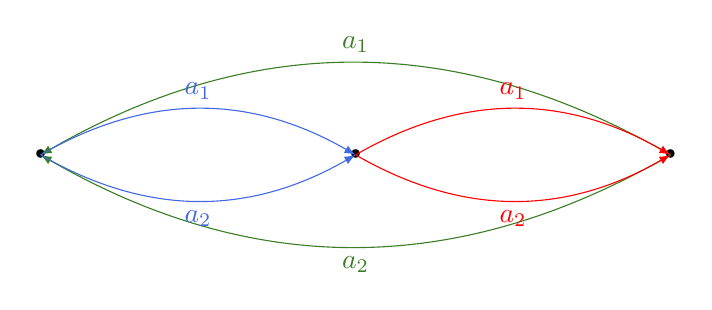
\begin{tikzpicture}
         \node[scale=0.8] (a) at (0, 0) {$\bullet$};
         \node[scale=0.8] (b) at (4, 0) {$\bullet$};
         \node[scale=0.8] (c) at (8, 0) {$\bullet$};
         \draw[->, >=latex, color = OliveGreen] (c.center) to[bend right] node[midway, above]{$a_1$} (a.center);
         \draw[->, >=latex, color = OliveGreen] (c.center) to[bend left] node[midway, below]{$a_2$} (a.center);
         \draw[->, >=latex, color = RoyalBlue] (a.center) to[bend left] node[midway, above]{$a_1$} (b.center);
         \draw[->, >=latex, color = RoyalBlue] (a.center) to[bend right] node[midway, below]{$a_2$} (b.center);
         \draw[->, >=latex, color = red] (b.center) to[bend left] node[midway, above]{$a_1$} (c.center);
         \draw[->, >=latex, color = red] (b.center) to[bend right] node[midway, below]{$a_2$} (c.center);
       \end{tikzpicture}
     \end{center}
     $X_H$ a $k$ sommets de degré $2n$ et a $\frac{k\cdot 2n}{2} = k\cdot n$ arêtes.
   \end{ex}

    
    
    


    
      
  




%%% Local Variables:
%%% mode: latex
%%% TeX-master: "../GAC_cours.tex" 
%%% End: